\documentclass[a4paper]{article}
\usepackage{amsfonts}
\usepackage{amsmath}
\usepackage{amssymb}
\usepackage{graphicx}     

\begin{document}
  
\noindent \large Auteur: Thijs Van Schel \\
\noindent \large Studierichting: Informatica\\
\noindent \large Oefeningenreeks 5D nr. 1.13\\

\medskip

\normalsize

$f(x) = \dfrac{x}{\sqrt{1+x^2}}$\\

$ = \displaystyle\int\limits_{-1}^{\sqrt{7}} \left|\dfrac{x}{\sqrt{1+x^2}}\right|dx$\\

$ = \displaystyle\int\limits_{-1}^{0} \dfrac{-x}{\sqrt{1+x^2}}dx + \displaystyle\int\limits_{0}^{\sqrt{7}}\dfrac{x}{\sqrt{1+x^2}}dx$\\

$u = 1+x^2, du = -2xdx$\\

$ \Rightarrow \displaystyle\int \dfrac{1}{2\sqrt{u}}du = \sqrt{u} + C = \sqrt{1+x^2} + C$\\

$ \Rightarrow \text{OPP} = [-\sqrt{1+x^2}]^0_{-1} + [\sqrt{1+x^2}]^0_{\sqrt{7}}$\\

$ = -1 + \sqrt{2} + 2\sqrt{2} - 1 = 3\sqrt{2} -2$\\


Tekening: \\

\begin{figure}[h]
\centering
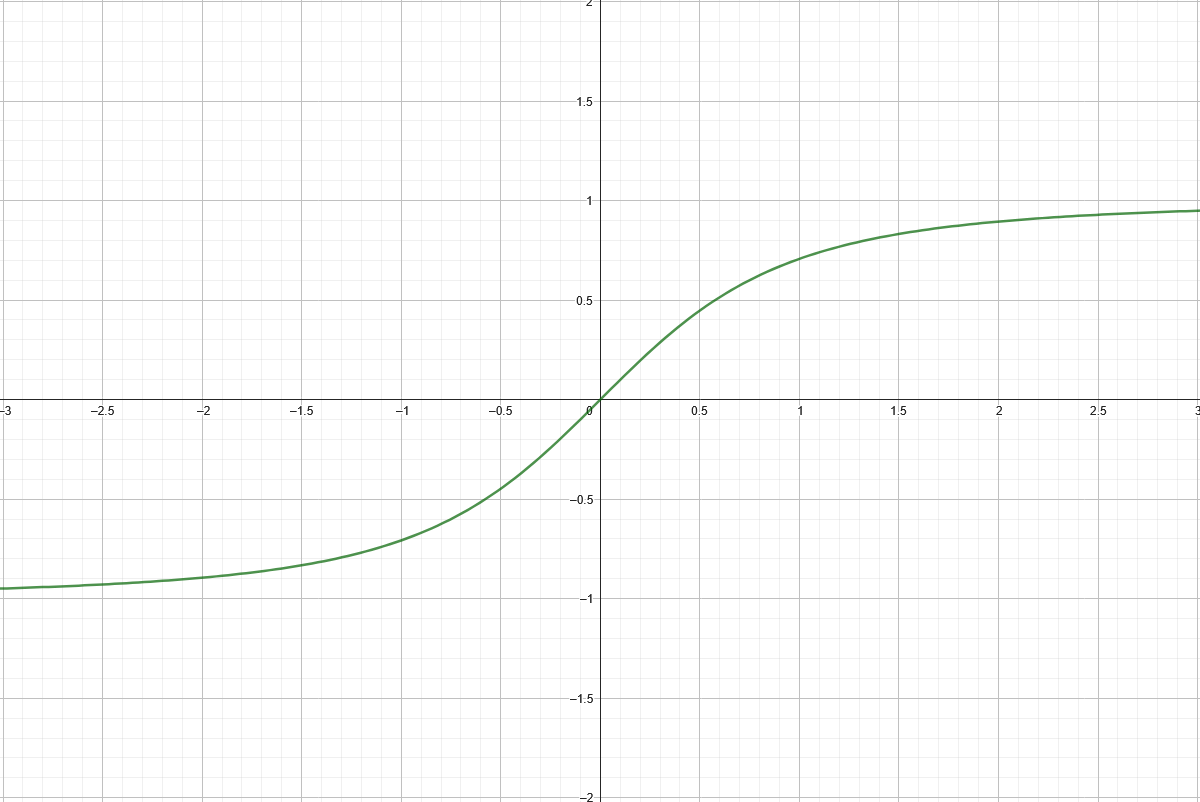
\includegraphics[width=0.5\linewidth]{5D-1.13-thijs.van.schel.INF.png}
\end{figure} 
\begin{thebibliography}{999}
%\bibitem{a} Referentie
\end{thebibliography}
\end{document} 
